%===============================================================================
% $Id: ifacconf.tex 19 2011-10-27 09:32:13Z jpuente $  
% Template for IFAC meeting papers
% Copyright (c) 2007-2008 International Federation of Automatic Control
%===============================================================================
\documentclass{ifacconf}
%\usepackage[cp1251]{inputenc}
%\usepackage[russian]{babel}
\usepackage{graphicx}      % include this line if your document contains figures
\usepackage{tikz}
\usepackage{natbib}        % required for bibliography
%\usepackage[ifacconf}

%===============================================================================
\begin{document}
\begin{frontmatter}

\title{On Local Optima Distribution in Buffer Allocation Problem for Production Line with Unreliable Machines\thanksref{footnoteinfo}} 
% Title, preferably not more than 10 words.

\thanks[footnoteinfo]{The research is supported by Russian Science Foundation  grant~21-41-09017.}

\author[First]{Alexandre Dolgui} 
\author[Second]{Anton Eremeev} 
\author[Third]{Viatcheslav Sigaev}

\address[First]{IMT Atlantique, Nantes, France}
\address[Second]{Sobolev Institute of Mathematics SB RAS, Novosibirsk, Russia (e-mail: eremeev@ofim.oscsbras.ru).}
\address[Third]{Avtomatika-Servis LLC, Omsk, Russia (e-mail: sigvs@yandex.ru).}


\begin{abstract}                % Abstract of not more than 250 words.
In this paper, we consider a buffer allocation problem in a manufacturing flow line, which has a series-parallel 
network structure where nodes correspond to buffers  of finite capacity, and arcs correspond to the machines. 
The machines are supposed to be unreliable, their time to failure and repair time are
assumed to be exponentially distributed. Different machines may have
different production rates and the production rates of all machines are assumed to be deterministic. 
The buffer allocation problem is 
in determine the capacities of all buffers with respect to a given
optimality criterion, which is a function of the average production rate
of the line, the buffer acquisition and installation cost and the
inventory cost. In our optimization algorithm, the tentative solutions are evaluated by means of an
approximate method based on the Markov models aggregation. We show that in many
problem instances, several clusters of local optima can be found and the ``massif central'' or ``big valley'' structure
of the fitness landscape is partially present. 
%The computational experiments show better quality of
%solutions obtained by a genetic algorithm with local search, compared to the multi-start 
%of a local search. 
The perfomance of genetic algorithms with respect to clusteres of the local optima is discussed.
\end{abstract}

\begin{keyword}
Production line, Unreliable machines, Buffer allocation, Series-parallel network, Genetic algorithms, Local optima.
\end{keyword}

\end{frontmatter}
%===============================================================================

\section{Introduction}

Buffer  capacity  allocation  problems  arise  in  a  wide  range  of  flow line manufacturing  systems, 
such  as  transfer  lines,  flexible  manufacturing  or  robotic  assembly  systems. 
The parts are accumulated in the intermediate buffers when the machines downstream are less productive than the upstream machines. 
In this paper, it is assumed that machines can break down and then go through repair. When a breakdown occurs, the corresponding 
machine is not used in production for a random repair time, and the length of this period is independent of the 
number of machines under repair. In this paper it is assumed  that there is a sufficient number of raw parts at 
the input of the system and the completed parts depart 
from the system immediately. One of the key performance measures of a flow-line is 
the average production rate, i.e., the expected number of parts produced per 
unit of time in the steady state mode.

Evaluation  of the manufacturing flow-line performance for given sizes of buffers is studied 
by~\cite{Proth84}, \cite{DG92}, \cite{Gershwin1993}, \cite{HPB1993}, \cite{Meerkov2009}, and \cite{TanGer09}. A number of
 models to evaluate the performance of lines with unreliable machines and fixed sizes of buffers were proposed by these and other authors. 
Markov models and aggregation or decomposition techniques are often used to calculate the
steady state throughput or other performance indicators for these lines.  
The  optimization  for  buffer  capacity  allocation with 
respect to diverse optimality criteria for different types of lines was studied 
using such models by \cite{SmiDas88}, \cite{So97}, \cite{GS}, \cite{Khelil_21}, \cite{ShiGer2009} and other authors. 

\subsection{The Buffer Allocation Problem Formulation} \label{bap_formulation}

In this paper, we consider the buffer allocation problem for lines with a series-parallel network. 
An example of a line, structured as a series-parallel network shown in Fig. ~\ref{lineexample}, where $M_1,…,M_7$ are machines and $B_0,…,B_5$ are buffers.

 \begin{figure}[h!]
	\centering
	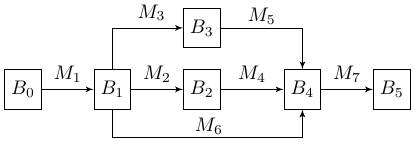
\includegraphics[scale=0.7]{LineSchems}
  \caption{Example of a line with a series-parallel network\label{lineexample}}
  \end{figure}

We assume that a machine can be in an operational state or under 
repair. An operational machine may be blocked and temporarily stopped in case if there 
is  no  room  in  the  downstream  buffer.  It  may  also  be  starved  if  there  are  no  parts  to 
process  in  the  upstream  buffer. Otherwise operational machines are working. In what 
follows, $m$ is the number of machines in a production line. A working machine $i$, 
$i=1,…,m$, is assumed to have a constant cycle time $C_i$ and, its average production 
rate $u_i=1/C_i$. 

It is supposed that machines may break down only when they are working. The times to fail 
and  times  to  repair  for  each  machine  are  assumed  to  be  mutually  independent  and 
exponentially distributed random values. Let $T_b^i$ denote the average time till failure, and let 
$\lambda_i=1/T_b^i$ be the failure rate for a machine $i$, $i=1,...,m$, conditioned that this machine is working. Similarly, let $T_r^i$ and $\mu_i=1/T_r^i$  
denote  respectively  the  time  to  repair  and  the repair rate for machine $i$, conditioned that this machine is under repair. Given the 
above  mentioned  assumptions,  the  system  has  the  steady  state  mode  (see  e.g. \cite{Seva62}),  and  the performance  of  the  system  in  this  mode  is  important  for 
applications.

%Let the buffers in the system be denoted by $B_1,…,B_n$ and l
Let $h_j$ be the capacity of buffer 
$B_j$, $j=1,\dots,n$.  Denote  the  vector  of  decision  variables  as  $H=  (h_1,  h_2,…, h_n )\in  Z_+^n$,  where  $Z_+$  is  the  set  of  non-negative  integers.  

The optimization criterion used in this paper is:
\begin{equation}
\label{criteria}
\max \phi(H)=T_{am} R(V(H)) - Q(H) - J(H),
\end{equation}
where 
\begin{itemize}
\item $T_{am}$  amortization time of the line (line life); 
\item $V(H)$  average production rate (steady state throughput); 
\item $R(V)$  revenue related to the production rate $V$; 
\item $J(H)$ cost of buffer configuration H; 
\item $d_j$ maximal admissible capacity of buffer $B_j$;
\item $Q(H)= c_1q_1(H)+ …+c_n q_n(H)$ average steady state inventory cost, where $q_j(H)$ is the average steady state number of parts in buffer $b_j$, for $j=1,…,n$.
\end{itemize}

The function $\phi(H)$ has to be maximized, subject to the constraints $h_1 \leq d_1$, $h_2 \leq d_2$,…, $h_n \leq d_n$.
The functions $R(V)$ and $J(H)$ are assumed to be monotone and  non-decreasing. 
The cost function $J(H)$ may be non-linear to model some standard buffer capacities or 
penalize  solutions  where  the  total  capacity  of  the  buffers  exceeds  an  upper  bound. A 
non-linear revenue function $R(V)$ can model the law of diminishing returns, for example, 
it  can  reflect  the  effect  of  overproduction  by  switching  from  strictly  increasing  to 
constant at a certain threshold. 
%A stepwise revenue function can be used to model zero 
%revenue  in  case  of  an  unacceptably  low  average  production  rate. 

%In general, the production rate with finite buffers is difficult to analyze precisely with 
%the Markov models. 
Exact performance computation of a production rate of a line with 
more than two machines and one buffer is problematic due to exponential growth of the 
number of states. Therefore, most of the techniques employed for the analysis of such 
systems are based on analytical approximations or simulations. Analytical 
approximations are generally based on the two-machines-one-buffer Markov models, 
and either aggregation~\cite{DeKoster87} or decomposition approach~\cite{DalXie89};~\cite{Gers87};~\cite{Li2005}. 
Simulation models are more expensive 
computationally but applicable to a wider class of systems (\cite{DS95};~\cite{SorJan2004}). 
 




In this paper, we use two-machines-one-buffer Markov model independently developed 
by~\cite{LP},~\cite{DF} and~\cite{Proth84}. For 
each tentative buffer allocation decision, the production rate is evaluated via an 
aggregation algorithm (\cite{Dolgui93};~\cite{DS95}), which is similar to the~\cite{TD87} techniques. 
This aggregation approach appears to be 
sufficiently rapid for evaluation of tentative buffer allocations within the optimization 
algorithms.  
 
The aggregation algorithm for production rate evaluation consists in recurrent 
replacement of two adjacent machines by a single machine. The parameters $\lambda^*$, $\mu^*$, $c^*$ of 
the resulting single machine are calculated from differential equations corresponding to
the two-machines-one-buffer Markov model. After $n$ steps of such aggregation 
procedure the system reduces to one virtual machine with parameters $\lambda^*$, $\mu^*$, $c^*$ and the 
estimate of the overall production rate $V(H)$ is given by $c^*\mu/(\lambda^*+\mu).$

The buffer allocation problem is known to be NP~hard as shown by~\cite{DEKS2013,DEKS2018}  and therefore it features some properties of the
well-known combinarotial optimization problems, one of such properties is that often it is easy to find a locally optimal solution (computable in polynomial time 
w.r.t. the problem input size), although it is hard to find the global optimum (requires exponential time in the worst case).  

\subsection{``Big Valley'' or ``Massif Central''}\label{subsec:landscapes}

In many combinatorial optimization problems, local optima of the objective function (or fitness)  tend to be clustered in a ``big valley`` (in  the case of minimization problems) or
``massif central`` (in  the case of maximization problems). This fitness landscape structure has been observed  e.g. in 
NK-landscapes by~\cite{KL87}, in the traveling salesman problem~(TSP) by~\cite{Boese,Hains}, in the graph bisection by~\cite{Boese}, and 
flowshop scheduling by~\cite{Reeves99}. More precisely, the ``big valley`` or
``massif central`` is described by the following two statements (see e.g.~\cite{Boese}):
\begin{enumerate}
\item Values of the objective function in the local optima tend to deteriorate with increasing distance to the global optimum (i.e. there is a correlation 
of objective function in the local optima with the distance to the global optimum).
\item Local optima are located relatively close both to each other and to the global optimum (they are located in a ball, which is smaller than 
the whole search space by several orders of magnitude).
\end{enumerate}
The presence of such structure partly explains good performance of genetic
algorithms~(GAs). If different local optima are found in the population of a GA and
the new solution is built by means of a crossover operator, 
then the intuition suggests that such algorithm should have good chances to find the
global optimum. This is supported by the theoretical analysis in the case of the Jump benchmark of~\cite{bib:Dang2016a}, and
by the experimental studies, e.g. of~\cite{Hains}.
In this respect, identification of the ``big valley`` or
``massif central`` structure, or the absence of such structure, is of great practical interest.

\subsection{Contribution of the Paper}
On the basis of computational experiments we show that the distribution of local optima for many instances of the buffer allocation 
problem on lines with a series-parallel structure has multiple clusters. The problem features causing such structures
are discussed. The ``massif central'' structure is identified but only in part: 
While the negative correlation between the objective function in local optima and their distance to the global solution is present, yet the 
concentration of all 
local optima in a tiny fraction of the search space is not confirmed. The observed structures of fitness landscape appear to be similar 
to those observed by~\cite{Hains} for the TSP, and in both cases the GA combined with a local search heuristic is able to locate
the cluster of high quality local optima.

\section{Investigation of Local Optima Properties} \label{investigation}

The distance to global optimum
in our case, we will calculate in the metric $l_1$.
To verify the ``massif central'' structure, we developed a method 
for finding the number of integer points in
a ball of a given radius at the intersection with a parallelepiped
whose faces are parallel to coordinate planes.
The method
was obtained by reducing the problem to a combinatorial
formulation, already considered earlier for the case of non-negative
integer points, using
generating functions, see~\cite{Sach}.

\subsection{Problem Instances Used In Computational Experiment}\label{subsec:tasks}
For computational experiments we use three series of problems:
\begin{table}[!ht]
\centering
\small
\begin{tabular}{|c|c|c|}
\hline
Series&Number of Lines&Number of Machines\\
\hline
AS & 8 & 4 -- 14 \\
BN & 10 & 5 \\
VP & 4 & 5 \\
\hline
\end{tabular}
\caption{List of series}\label{tabl:series}
\vspace{-0.5cm}
\end{table}

The AS series consists of instances created from lines~1,2,6,7,8 from~\cite{Ancelin1987} with real data from
Renault production.
A distinctive feature of the 7 and 8 lines is the presence
parallel sections (see figures~\ref{fig:vis_as7},~\ref{fig:vis_as8}).
Line parameters~1,2,6,7,8 are given in tables \ref{tabl:as1}-\ref{tabl:as8}.

 \begin{figure}[h!]
	\centering
	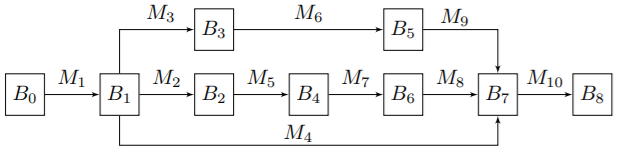
\includegraphics[scale=0.6]{ans7}
  \caption{Line structure AS7} \label{fig:vis_as7}
  \end{figure}

 \begin{figure}[h!]
	\centering
	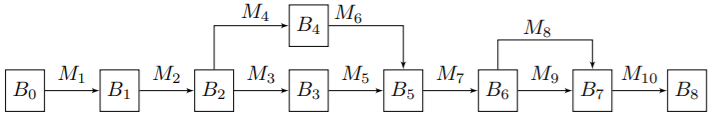
\includegraphics[scale=0.55]{ans8}
  \caption{Line structure AS8} \label{fig:vis_as8}
  \end{figure}


\begin{table}[h!]
\centering
\small
\begin{tabular}{||c|c||c|c|c|c||}
\hline \multicolumn{2}{||c||}{buffers}&\multicolumn{4}{|c||}{machines}\\
\hline
$i$ & $d_i$ & $j$ & $T^{\rm O}_j$ & $T^{\rm B}_j$ & $U_i$\\
\hline
1 & 20 & 1 & 244.2 & 150 & 10\\
2 & 17 & 2 & 255.3 & 300 & 10\\
3 & 38 & 3 & 176 & 75 & 10\\
4 & 48 & 4 & 184 & 600 & 10\\
&& 5 & 192 & 450 & 10\\
\hline
\end{tabular}\\
\caption{Problem parameters $\textit{AS1}$}\label{tabl:as1}
\end{table}

\begin{table}[h!]
	\centering
	\small
	\begin{tabular}{||c|c||c|c|c|c||}
		\hline
		\multicolumn{2}{||c||}{Buffers}&\multicolumn{4}{|c||}{Machines}\\
		\hline
		$i$ & $d_i$ & $j$  & $T^{\rm O}_j$ & $T^{\rm B}_j$ & $U_i$ \\
		\hline
		1 & 0   & 1  & 10000 & 440 & 22 \\
		2 & 50  & 2  & 20000 & 440 & 23 \\
		3 & 20  & 3  & 5000  & 430 & 22 \\
		4 & 50  & 4  & 40000 & 520 & 23 \\
		5 &  0  & 5  & 30000 & 430 & 24 \\
		6 & 80  & 6  & 2442  & 440 & 22 \\
		7 & 20  & 7  & 1840  & 520 & 23 \\
		8 & 100 & 8  & 1680  & 430 & 21 \\
		9 & 100 & 9  & 2208  & 920 & 24 \\
		\hline
	\end{tabular}
	\caption{Problem parameters $\textit{AS2}$} \label{tabl:as2}
\end{table}  
\begin{table}[h!]
	\centering
	\small
	\begin{tabular}{||c|c||c|c|c|c||}
		\hline 
		\multicolumn{2}{||c||}{Buffers}&\multicolumn{4}{|c||}{Machines}\\
		\hline
		$i$ & $d_i$ & $j$  & $T^{\rm O}_j$ & $T^{\rm B}_j$ & $U_i$ \\
		\hline
		1  & 60 & 1 & 29880 & 22000 &  385\\
		2  & 60 & 2 & 29880 & 22000 & 426\\
		3  & 50 & 3 & 876000 & 22300 & 330 \\
		4  & 70 & 4 & 29880 & 22000 & 372\\
		5  & 60 & 5 & 33250 & 27500 & 316 \\
		6  & 80 & 6 & 144000 & 8500 & 340 \\
		7  & 45 & 7 & 102300 & 74000 & 340 \\
		8  & 25 & 8 & 113300 & 7200 & 340 \\
		9  & 35 & 9 & 540000 &  60000 & 380 \\
		10 & 80 & 10 & 538800 & 349000 & 350 \\
		11 & 40 & 11 & 5064000 & 73700 & 400 \\
		12 & 45 & 12 & 468000 & 306000 & 400 \\
		13 & 65 & 13 & 1032000 & 54000 & 319 \\
		& & 14 & 45600 & 31120 & 319 \\
		\hline
	\end{tabular}
	\caption{Problem parameters $\textit{AS6}$} \label{tabl:as6}
\end{table}  

\begin{table}[h!]
	\centering
	\small
	\begin{tabular}{||c|c||c|c|c|c||}
		\hline 
		\multicolumn{2}{||c||}{Buffers}&\multicolumn{4}{|c||}{Machines}\\
		\hline
		$i$ & $d_i$ & $j$  & $T^{\rm O}_j$ & $T^{\rm B}_j$ & $U_i$ \\
		\hline
		1 & 15 & 1 & 50000 & 12000 & 1000\\
		2 & 10 & 2 & 48000 & 2000 & 3450\\
		3 & 15 & 3 & 55000 & 9000 & 2780 \\
		4 & 10 & 4 & 39000 & 6000 & 3030\\
		5 &  25  & 5 & 75000 & 10000 & 3333\\
		6 &  10 & 6 & 59000 & 11000 & 2560\\
		7 & 10 & 7 & 28000 & 8000 & 3030\\
			&  & 8 & 35000 & 8000 & 3125\\
			&  & 9 & 65000 &  35000 & 2174\\
			&  & 10 & 20000 & 4000 & 800\\
		\hline
	\end{tabular}
	\caption{Problem parameters $\textit{AS7}$} \label{tabl:as7}
\end{table}
\begin{table}[h!]
	\centering
	\small
	\begin{tabular}{||c|c||c|c|c|c||}
		\hline
		\multicolumn{2}{||c||}{Buffers}&\multicolumn{4}{|c||}{Machines}\\
		\hline
		$i$ & $d_i$ & $j$  & $T^{\rm O}_j$ & $T^{\rm B}_j$ & $U_i$ \\
		\hline
		1 & 1300 & 1 & 87000 & 27000 & 23\\
		2 & 200 & 2 & 77000 & 22000 & 27\\
		3 & 0 & 3 & 580000 & 18000 & 38\\
		4 & 0 & 4 & 410000 & 12500 & 30\\
		5 & 0 & 5 & 580000 & 18000 & 38\\
		6 & 2000 & 6 & 410000 & 12500 & 30\\
		7 & 0 & 7 & 725000 & 21000 & 20\\
		  &  & 8 & 550000 & 14000 & 40\\
		 &  & 9 & 430000 & 24000 & 43\\
		   &  & 10 & 270000 & 22000 & 33\\
		\hline
	\end{tabular}
	\caption{Problem parameters $\textit{AS8}$} \label{tabl:as8}
\end{table}

Instances bn5.1-bn5.10 consist of 10 lines from~\cite{eng1} with $m=5$. There are two bottlenecks in each line. By
bottleneck we mean here a line section of two relatively slow machines and a buffer
between them. 

Problems vp6.9-vp6.10, vp7.9-vp7.10 are defined on serial five-machine lines of~\cite{vp}. 


\subsection{Computational Experiment} \label{subsec:experiment}

A series of experiments were carried out on existing instances for
determination of the landscape structure. 
To find a local optimum, we used the local search algorithm LSA. At each iteration, the LSA searches through the neighborhood of radius 1 in metric $l_1$ around
the current solution. If an improving feasible solution in terms of the  objective function is found in the neighborhood, then it becomes the new current solution.
The process continues as long as an improvement can be found.  Starting from any feasible solution, the LSA
moves iteratively to a local optimum, i.e. a solution that does not have an improving neighbour within the radius~1 in metric $l_1$.

In each run of the local search algorithm LSA, it starts at a randomly generated solution $H$ whose elements $h_i$ are chosen with
uniform distribution between 1 and $d_i$.
This procedure was repeated 300 times to create the necessary
sample size (\cite{Boese}). Based on this sample, we calculated the total
number of admissible solutions $|\Omega |$ in the minimal ball encompassing all the
local optima found. In our case, the ball was chosen in the metric $l_1$, with the center in the best found local optimum.

In table~\ref{spher_as}-\ref{spher_bn} the column $V1$ contains the cardinality $| \Omega |$ for balls containing
local optima, the column $V2$ contains cardinality of the entire space of feasible
solutions, and the column $V1/V2$ is the ratio of the two.
As can be seen from the tables, the second part of the massif central / big valley conjecture was not 
confimed and in most of the instances under consideration
the optima are scattered throughout the solution space.

\begin{table}[ht]
	\centering
	\begin{tabular}{|c|c|c|c|}
		\hline
		\hspace*{0.1cm} instance \hspace*{0.1cm} &
		\hspace*{0.1cm}$V1$\hspace*{0.1cm}&
		\hspace*{0.1cm}$V2$\hspace*{0.1cm}&
		\hspace*{0.1cm}$V1/V2$\hspace*{0.1cm}\\
		\hline
		1 &  2,84E+05  &  5,74E+05 &   0,49\\
		2 &  8,88E+11  &  9,48E+11 &   0,94\\
		3 &  8,60E+01  &  4,85E+03 &   0,02\\
		4 &  2,34E+22  &  2,89E+22 &   0,81\\
		5 &  4,17E+07  &  9,75E+07 &   0,43\\
		6 &  1,00E+00  &  5,23E+08 &   0,00\\
		\hline
	\end{tabular}
	%\vspace{1em}
	\caption{Results of running a local search multiple times for a series as.1 - as.6}	\label{spher_as}
\end{table}
\begin{table}[ht]
	\centering
	\begin{tabular}{|c|c|c|c|}
		\hline
		\hspace*{0.1cm}instance \hspace*{0.1cm} &
		\hspace*{0.1cm}$V1$\hspace*{0.1cm}&
		\hspace*{0.1cm}$V2$\hspace*{0.1cm}&
		\hspace*{0.1cm}$V1/V2$\hspace*{0.1cm}\\
		\hline
		9  & 7,97E+03  &  1,00E+04  &  0,80\\
		10 & 7,55E+03  &  1,46E+04  &  0,52\\
		\hline
	\end{tabular}
	%\vspace{1em}
	\caption{Results of running a local search multiple times for the series vp6.9 - vp6.10}	\label{spher_vp6}
\end{table}
\begin{table}[ht]
	\centering
	\begin{tabular}{|c|c|c|c|}
		\hline
		\hspace*{0.1cm}instance \hspace*{0.1cm} &
		\hspace*{0.1cm}$V1$\hspace*{0.1cm}&
		\hspace*{0.1cm}$V2$\hspace*{0.1cm}&
		\hspace*{0.1cm}$V1/V2$\hspace*{0.1cm}\\
		\hline
		9  & 6,50E+03  &  1,00E+04  &  0,65\\
		10 & 9,95E+03  &  1,46E+04  &  0,68\\
		\hline
	\end{tabular}
	%\vspace{1em}
	\caption{Results of running a local search multiple times for the series vp7.9 - vp7.10}	\label{spher_vp7}
\end{table}

The first part of the massif central / big valley conjecture about the correlation $\rho(\varphi(\xi),r(\xi,\xi^*))$ of the value of 
objective function of local optima $\varphi(\xi)$
with the distance $r(\xi,\xi^*)$ to a global optimum. 
Our experiments suggest that there is a negative correlation $\rho$, and all values of the
correlation are significantly different from 0 with a confidence level of 95\% (tables~\ref{res_korr_as_vp}--\ref{res_korr_bn_vp}).
\begin{table}[h!]
	\vspace{1cm}
	\centering
	\begin{tabular}{|c|c|c|c|}
		\hline
		\hspace*{0.1cm}instance \hspace*{0.1cm} &
		\hspace*{0.1cm}$V1$\hspace*{0.1cm}&
		\hspace*{0.1cm}$V2$\hspace*{0.1cm}&
		\hspace*{0.1cm}$V1/V2$\hspace*{0.1cm}\\
		\hline
		1 &  1,44E+05  &  1,94E+05  &  0,74\\
		2 &  9,96E+03  &  1,94E+05  &  0,05\\
		3 &  9,07E+04  &  1,94E+05  &  0,47\\
		4 &  2,06E+04  &  1,94E+05  &  0,11\\
		5 &  6,95E+04  &  1,94E+05  &  0,36\\
		6 &  6,94E+04  &  1,94E+05  &  0,36\\
		7 &  2,45E+04  &  1,94E+05  &  0,13\\
		8 &  3,42E+03  &  1,94E+05  &  0,02\\
		9 &  6,28E+04  &  1,94E+05  &  0,32\\
		10&  1,00E+00  &  1,94E+05  &  0,00\\
		\hline
	\end{tabular}
	\vspace{1em}
	\caption{Results of 300 runs the local search  for the series bn5.1 - bn5.10}	\label{spher_bn}
\end{table}
\begin{table}[h!]
	\centering
	\begin{tabular}{|c|c|}
		\hline
		%\hspace*{2mm} № \hspace*{2mm} & \hspace*{5.1cm} $\rho(r(\xi, \xi*),\varphi(\xi))$\hspace*{5.1cm}\\
		\hspace*{2mm} instance \hspace*{2mm} & \hspace*{1cm} $\rho(r(\xi, \xi*),\varphi(\xi))$\hspace*{1cm}\\
		\hline
		\multicolumn{2}{|c|}{Series as.1 - as.5}\\
		\hline
		1  & -0,87078206\\
		2  & -0,437208613\\
		7  & -0,547348483\\
		8  & -0,943725905\\
		\hline
		\multicolumn{2}{|c|}{Series vp6.9 - bn6.10}\\
		\hline
		9  & -0,833583818\\
		10 & -0,778237651\\
		\hline	
	\end{tabular}
	\vspace{1em}
	\caption{Results of 300 runs of the local search for series $as$ and $vp6$}	\label{res_korr_as_vp}
\end{table}

\begin{table}[h!]
	\centering
	\begin{tabular}{|c|c|}
		\hline
		\hspace*{2mm} instance \hspace*{2mm} & \hspace*{1cm} $\rho(r(\xi, \xi*),\varphi(\xi))$\hspace*{1cm}\\
		\hline
		\multicolumn{2}{|c|}{Series bn5.1 - bn5.9}\\
		\hline
		1  & -0,706451573\\
		2  & -0,872602935\\
		3  & -0,914939714\\
		4  & -0,999969666\\
		5  & -0,972555479\\
		6  & -0,729655068\\
		7  & -0,973827419\\
		8  & -0,846807033\\
		9  & -0,884916669\\
		\hline
		\multicolumn{2}{|c|}{Series vp7.9 - bn7.10}\\
		\hline
		9  & -0,907792301\\
		10 & -0,889724863\\		
		\hline		
	\end{tabular}
	\vspace{1em}
	\caption{Correlation $\rho(\varphi(\xi),r(\xi,\xi^*))$ in series $bn$ and $vp7$}	\label{res_korr_bn_vp}
\end{table}

An interesting fact is 
that in problems as.4, bn5.1, the entire set of local optima splits
into clusters, and in each of the clusters, the negative correlation~$\rho$ is observed.
%for each of which a part of the thesis about tendency to
%deterioration of the value of the objective function of local optima
%with increasing distance to global optimum.

Figures~\ref{fig:multistart_klaster} and ~\ref{klaster_bn5_1} show diagrams of local optima for problems
as.6, bn5.1, where the ordinate shows the value of objective function of local optimum $\varphi(H)$, and the abscissa is
distance in metric $l_1$ to the best found solution.

Clustering effect is especially well manifested in instances with parallel sections of line.
This effect can be justified by the  fact that there are several different paths in lines with a parallel structure.
from start buffer to end buffer. Thus, if there are two parallel paths that are identical in their network structure,
such that one path will have relatively large buffers, and other one will have relatively small buffers, then 
it is possible to obtain two solutions with close values of the objective function, but located at a large distance from each other.

 \begin{figure}[h!]
	\centering
	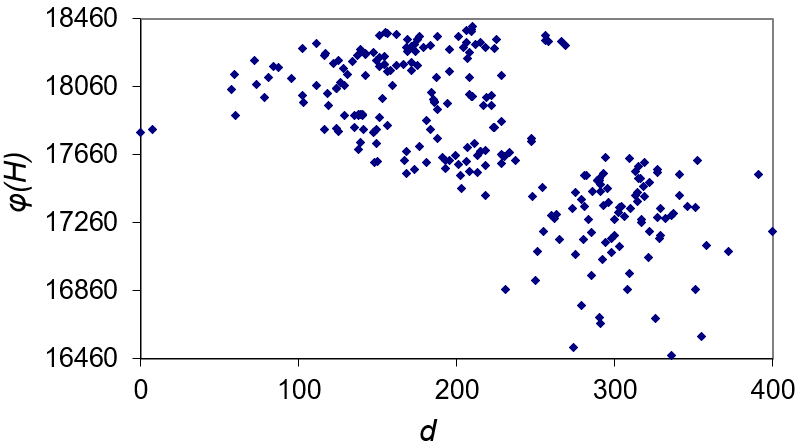
\includegraphics[scale=0.5]{multistart_klaster}
  \caption{The set of local optima obtaained in as.4 } \label{fig:multistart_klaster}
  \end{figure}
\begin{figure}[h!]
	\begin{center}
		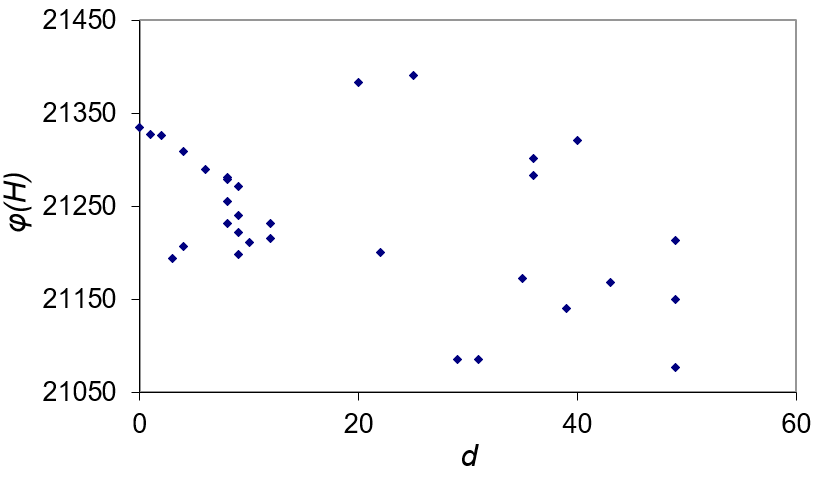
\includegraphics[scale=0.5]{klaster_bn5_1.png}\\
		\caption{The set of  local optima obtained in bn5.1.} \label{klaster_bn5_1}
	\end{center}
\end{figure} 

Another reason for clustering effect is the property of
line symmetry. This property is indicated by~\cite{LP} for a serial line,
consisting of two machines and a buffer
between them. If we swap the parameters of the first and the second machines so 
that the input buffer of the line will become its output, and the output buffer will become the input, then
line performance will not change.

Consider the example of serial line t.1 of
%{\frac{1}{T^{\rm O}_j} = 2U_j}, {\frac{1}{T^{\rm B}_j}= 4U_j}, {U_j = U_{j+1} }
three machiness and two buffers between them with the following parameters: ${T^{\rm O}_i=T^{\rm B}_i=1}$, $i = 1,\ldots,3$;
 ${U_1=1}$, ${U_2=0.5}$ , ${U_3=1}$;
 ${d_j=4}$, ${c_j=0}$, $j = 1,\ldots,2$;
 $T_{am}=7000$;
 $J(H)=50\cdot(h_1+h_2)$;
 if $V(H) < 2570$ then $R(V(H))=0.9\cdot V(H)$, otherwise $R(V(H))=2570$.

 \begin{figure}[h!]
	\centering
	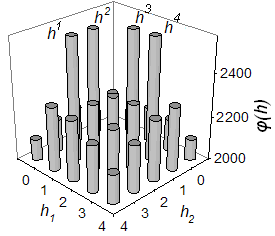
\includegraphics[scale=0.7]{test}
  \caption{Values of the objective function on the set $D$ for problem t.1\label{t_1}}
  \end{figure}

The set of global optima (see Fig.~\ref{t_1}) of this example splits into two clusters. The
first cluster contains solutions $H^1=(1,2)$ and $H^2=(1,3)$, and
the second is the solutions $H^3=(2,1)$ and $H^4=(3,1)$. Clustering of the optima in
this example is a consequence of the line symmetry effects
%and singularities
in the aggregation algorithm from~\cite{Dolgui93, DF}, which is used to calculate the line performance.

In the general case, for lines with $n\geq 3$ buffers, the effect of
symmetry can be observed in several internal areas of a
line. As a consequence, with this aggregation algorithm, a
set of local optima may be divided into several clusters.

%If a buffer allocation problem has local optima with different values of objective 
%function, then it can become difficult for local search algorithm.
A sequence of points generated by an algorithm, based on the local search principles, after falling into one of the clusters, usually
 remains in the cluster until the end of the calculations. For example, for a tabu-search algorithm, transition between clusters is unlikely, which also makes
such tasks difficult for it. 
%Best performance for
%considered problems, compared with the other two algorithms,
%showed the 
The GA with local optimization heuristic from~\cite{sHBBA2007} is one of the most efficient algorithms for this problem. 
As experiments have shown, the population of the pure GA contains individuals that correspond to solutions from different clusters. 
Usage of selection, crossover and mutation operators allows maintaining the diversity of population.
There is a competition between different clusters for their representation in the population at each step of a GA.

 \begin{figure}[h!]
%	\centering
	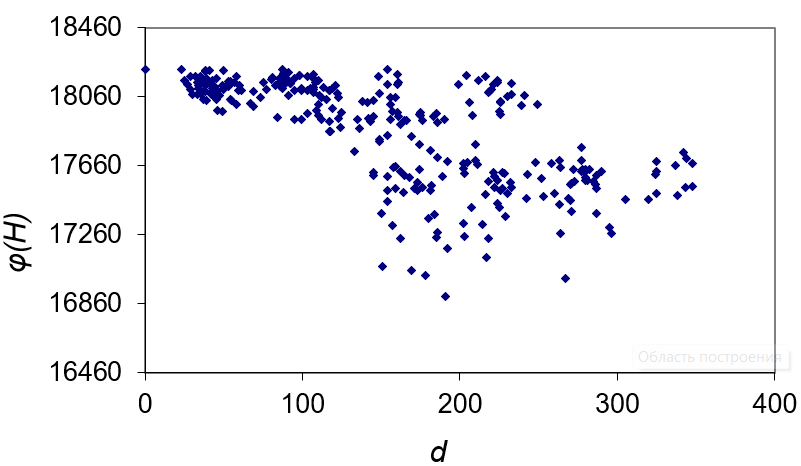
\includegraphics[scale=0.5]{ga_klaster}
  \caption{Final population of GA on instance as.4} \label{fig:ga_klaster}
  \end{figure}
 \begin{figure}[h!]
\centering
	\hspace{1.6em} 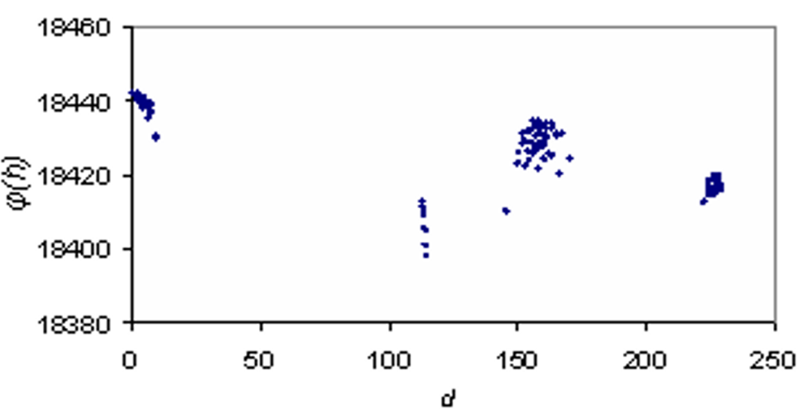
\includegraphics[scale=0.5]{gals_klaster}
%	\centering
%	\hspace{1.6em} 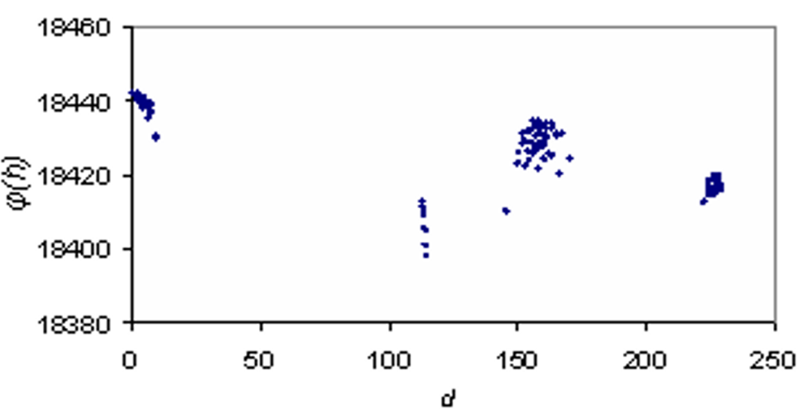
\includegraphics[width=5.3cm, height=3.5cm]{gals_klaster}
  \caption{Final population of the GA with local optimization heuristic on instance as.4 \label{fig:gals_klaster} 
  (note that the scale of both axes is different from 
  Figs~\ref{fig:multistart_klaster} and \ref{fig:ga_klaster})}
  \end{figure}

Problem as4 can serve as an illustrative example. Fig.~\ref{fig:multistart_klaster} shows the structure 
of the set of local optima obtained by multistart  of the local search. 
Figures~\ref{fig:ga_klaster} and~\ref{fig:gals_klaster} show the final populations of the pure GA and the GA 
with local optimization heuristic, where the multi-cluster structure of the final population is visible. 
Figure~\ref{fig:gals_klaster} shows the impact of the local heuristic in the GA: with this heuristic only the best individuals 
of the top four clusters from Fig.~\ref{fig:ga_klaster} are present.

%\section{Conclusion}
%
%\begin{enumerate}
%
%\item Cluster structure of local optima is established of some tasks having parallel parts in structure.
%
%\item Reasons for the emergence of clusters of local optima are determined.
%
%\end{enumerate}

\bibliography{eremeev_et_al}   
                                                  
\end{document}


